%Template Presentation in LaTeX
%Departemen Teknik Elektro dan Informatika
%Sekolah Vokasi UGM

%Dikembangkan oleh Dr. Ir. Fahmizal, S.T., M.Sc. dan Tim

%Perangkat lunak yang digunakan untuk mengolah LaTeX pada template ini adalah
%- TeXstudio
%- MiKTex
%- Overleaf (LaTEX editor berbasis daring)


\documentclass [xcolor={dvipsnames}, t] {beamer} 
\usepackage[utf8]{inputenc}
\usepackage{booktabs, comment} 
\usepackage[absolute, overlay]{textpos} 
\usepackage{pgfpages}
\usepackage[font=footnotesize]{caption}
\useoutertheme{infolines} 
\usepackage[orientation=landscape,size=custom,width=16,height=9,scale=0.4,debug]{beamerposter} 

\definecolor{gold}{RGB}{254, 206, 0}
\setbeamercolor{title in head/foot}{bg=gold, fg=black}
\setbeamercolor{author in head/foot}{bg=myuniversity}
\setbeamertemplate{page number in head/foot}{}
\usepackage{csquotes}
\usepackage{amsmath}
\usepackage[makeroom]{cancel}
\usepackage{multirow}
\usepackage{breqn}
\usepackage{animate}
\usepackage{movie15}			
\usepackage{textpos}
\usepackage{tikz}
\usetikzlibrary{positioning}
\usepackage{array}
\usepackage{siunitx}
\usepackage{tikz}
\usetheme{Madrid}
\definecolor{myuniversity}{RGB}{0, 85, 150}
\usecolortheme[named=myuniversity]{structure}
\usepackage{tikz}

%paket untuk bibTex
\usepackage{cite}
\bibliographystyle{IEEEtran}

% set colors
\definecolor{myNewColorA}{RGB}{0, 0, 128} %{46, 162, 151}
\definecolor{myNewColorB}{RGB}{253, 203, 44} %{255, 235, 59}
\definecolor{myNewColorC}{RGB}{253, 203, 44} % {130,138,143}
\setbeamercolor*{palette primary}{bg=myNewColorC}
\setbeamercolor*{palette secondary}{bg=myNewColorB, fg = white}
\setbeamercolor*{palette tertiary}{bg=myNewColorA, fg = white}
\setbeamercolor*{titlelike}{fg=myNewColorA}
\setbeamercolor*{title}{bg=myNewColorA, fg = white}
\setbeamercolor*{item}{fg=myNewColorA}
\setbeamercolor*{caption name}{fg=myNewColorA}
\usefonttheme{professionalfonts}

% Code colors (Irrelevant from the presentation color theme!)
\definecolor{codemaincolor}{RGB}{0, 0, 0}
\definecolor{codebackgroundcolor}{RGB}{255, 255, 255}
\definecolor{codekeywordcolor}{RGB}{0, 0, 255}
\definecolor{codestringcolor}{RGB}{163, 21, 21}
\definecolor{codecommentcolor}{RGB}{39, 139, 39}
\definecolor{codeusertypecolor}{RGB}{43, 145, 175}

\usepackage{listings}
\usepackage{lstautogobble}
\lstset {
	basicstyle={\scriptsize \ttfamily \color{codemaincolor}},
	backgroundcolor=\color{codebackgroundcolor},
	autogobble = true,
	tabsize = 2,
	xleftmargin=0pt,
	xrightmargin=0pt,
	aboveskip=0pt, % \medskipamount,
	belowskip=0pt, % \medskipamount,
	literate={\ \ }{{\ }}1
}

\lstset{ 
	language=Matlab,                		% choose the language of the code
	%basicstyle=10pt,       				% the size of the fonts that are used for the code
	%numbers=left,                  			% where to put the line-numbers
	%numberstyle=\footnotesize,      		% the size of the fonts that are used for the line-numbers
	%stepnumber=1,                   			% the step between two line-numbers. If it's 1 each line will be numbered
	%numbersep=5pt,                  		% how far the line-numbers are from the code
	%	backgroundcolor=\color{white},  	% choose the background color. You must add \usepackage{color}
	showspaces=false,               		% show spaces adding particular underscores
	showstringspaces=false,         		% underline spaces within strings
	showtabs=true,                 			% show tabs within strings adding particular underscores
	frame=single,	                			% adds a frame around the code
	tabsize=2,                				% sets default tabsize to 2 spaces
	%	captionpos=b,                   			% sets the caption-position to bottom
	breaklines=true,                			% sets automatic line breaking
	breakatwhitespace=false,        		% sets if automatic breaks should only happen at whitespace
	escapeinside={\%*}{*)}          		% if you want to add a comment within your code
}

\lstdefinestyle{C++} {
	language=C++,
	otherkeywords = {final, override, noexcept},
	keywordstyle = {\color{codekeywordcolor}},
	stringstyle = {\color{codestringcolor}},
	commentstyle = {\color{codecommentcolor}\em},
	% Class and types highlighting
	classoffset=1, % starting new class
	morekeywords={vector, ostream, unique_ptr, shared_ptr, T, device_t, abstract_device, device_one, device_two, device_three, executable_device, measurable_device, my_device, concept_t, model, device_one_model, device_two_model, sensor_t, history_t},
	keywordstyle=\color{codeusertypecolor},
	classoffset=0,
}


\title[ugm.ac.id]{Identification Model Motor DC}
\subtitle{(Ini adalah contoh template PPT dengan LaTex)}
\titlegraphic{
\includegraphics[height=1cm]{logougm.png}}
\author[locally rooted, globally respected]{Presented by \\ Dr. Ir. Fahmizal, S.T., M.Sc.}


\institute[]{Teknologi Rekayasa Instrumentasi dan Kontrol
	\\Departemen Teknik Elektro dan Informatika 
	\\Sekolah Vokasi, Universitas Gadjah Mada}
\date{\today}


\addtobeamertemplate{navigation symbols}{}{%
    \usebeamerfont{footline}%
    \usebeamercolor[fg]{footline}%
    \hspace{1em}%
    \insertframenumber/\inserttotalframenumber}

\begin{document}
\begin{frame}
\maketitle
\end{frame}


\logo{
\includegraphics[scale=0.2]{logougm.png}~}


\begin{frame}
\frametitle{Outline}
\tableofcontents
\end{frame}

\section{Introduction}


\begin{frame}
	\frametitle{Pendahuluan}
	\framesubtitle{Pengertian Motor DC}
	\begin{columns}[T]% align columns
		\begin{column}{0.4\textwidth}
			
			\color{black}\rule{\linewidth}{4pt}
			
			Motor DC atau dalam bahasa Indonesia disebut motor arus searah adalah ....
		\end{column}%
		\hfill%
		\begin{column}{0.5\textwidth}
			\color{myNewColorA}\rule{\linewidth}{4pt}
			Ilustrasi Motor DC:\newline
			\animategraphics[loop,width=5cm]{7}{animate/PMDC/PMDC-}{0}{3}
		\end{column}
	\end{columns}
\end{frame}


	\begin{frame}{Struktur Fisik}
	\begin{columns}[T] % align columns
		\begin{column}{0.48\textwidth}
			Parameter:
			\color{black}\rule{\linewidth}{4pt}
			\begin{flushleft}
				\begin{tabular}{lll}
					$J$ &:& Momen inersia rotor $(Kg.m^2)$\\
					$b$ &:& Koefisien gaya gesek viskos $(N.m.s)$\\
					$Ke$ &:& Koefisien gaya elektromotif $(V/rad/sec)$\\
					$Kt$ &:& Koefisien torsi motor $(N.m/Amp)$\\
					$R$ &:& Resistansi kumparan $(Ohm)$\\
					$L$ &:& Induktansi kumparan $(H)$\\
				\end{tabular}
			\end{flushleft}
		\end{column}%
		\hfill%
		\begin{column}{0.48\textwidth}
			Skematik Motor DC:\newline
			\color{myNewColorA}\rule{\linewidth}{4pt}
			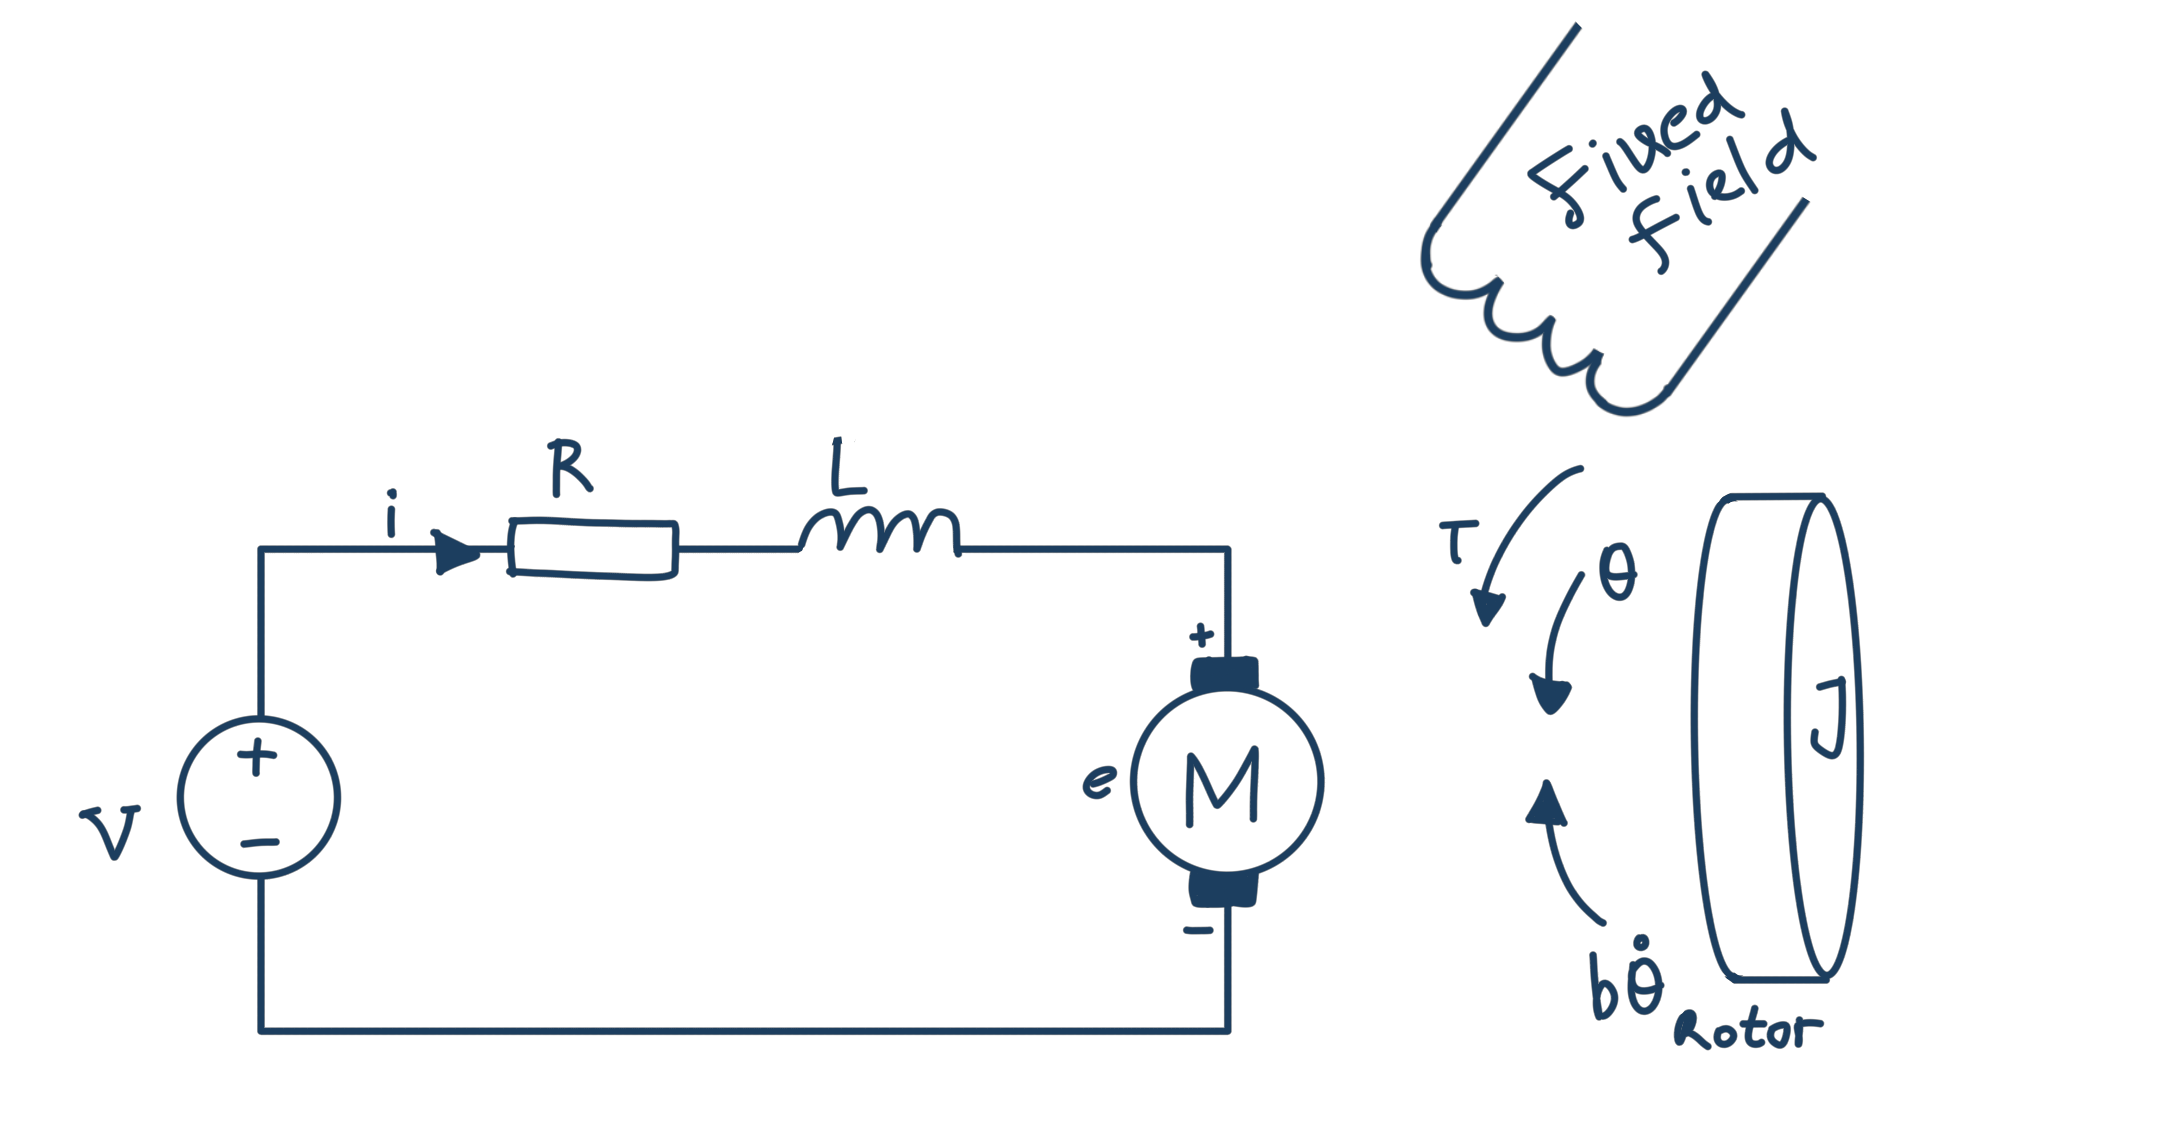
\includegraphics[width=7.5cm]{fig/skematik motor dc.png}
		\end{column}
	\end{columns}
\end{frame}


\section{Diagram Blok Sistem}


\begin{frame}
	\frametitle{Diagram Blok Plant Motor DC}
	\framesubtitle{Struktur motor DC:}
	
	\begin{center}
		\begin{tikzpicture}
			% Sum shape
			\node[draw, circle, minimum size=0.6cm, fill=Rhodamine!50] (sum) at (0,0){};
			
			\draw (sum.north east) -- (sum.south west)
			(sum.north west) -- (sum.south east);
			
			\draw (sum.north east) -- (sum.south west)
			(sum.north west) -- (sum.south east);
			
			\node[left=-1pt] at (sum.center){\tiny $+$};
			\node[below] at (sum.center){\tiny $-$};
			
			% Controller
			\node [draw, fill=Goldenrod, minimum width=2cm, minimum height=1.2cm, right=1cm of sum] (controller) {\large $\frac{1}{Ls+R}$};
			
			\node [draw, minimum width=1cm, minimum height=0.6cm, below=0.3cm of controller] (text1) {\textit{Electrical}};
			
			% System H(s)
			\node [draw, fill=SpringGreen, minimum width=1cm, minimum height=1cm, right=1.5cm of controller] (system1) {$Kt$};
			
			\node [draw, fill=Aquamarine, minimum width=2cm, minimum height=1.2cm, right=4cm of controller] (system2) {\large $\frac{1}{Js+b}$};
			
			\node [draw, minimum width=1cm, minimum height=0.6cm, below=0.3cm of system2] (text2) {\textit{Mechanical}};
			
			% Sensor block
			\node [draw, fill=SeaGreen, minimum width=1cm, minimum height=1cm,  below right= 1.5cm and 1.5cm of controller]  (sensor) {$Ke$};
			
			% Arrows with text label
			\draw[-stealth] (sum.east) -- (controller.west);
			
			\draw[-stealth] (controller.east) -- (system1.west) 
			node[midway,above]{$I(s)$};
			
			\draw[-stealth] (system1.east) -- (system2.west) 
			node[midway,above]{$T(s)$};
			
			\draw[-stealth] (system2.east) -- ++ (1.25,0) 
			node[midway](output){}node[midway,above]{$\dot{\theta}(s)$};
			
			\draw[-stealth] (output.center) |- (sensor.east);
			
			\draw[-stealth] (sensor.west) -| (sum.south) 
			node[very near start,above]{$e(s)$};
			
			\draw (sum.west) -- ++(-1,0) 
			node[midway,above]{$V(s)$};
		\end{tikzpicture}
	\end{center}
\end{frame}

\begin{frame}{Fungsi Alih}
	Diagram blok \textit{plant} motor DC menghasilkan persamaan fungsi alih berikut:
	\begin{equation}
		\frac{\dot{\theta}(s)}{V(s)}=\frac{Kt}{(Js+b)(Ls+R)+KtKe} \qquad \left[\frac{rad/sec}{V}\right] 
	\end{equation} 
	Persamaan di atas merupakan fungsi alih kecepatan motor DC. Dengan mengintegralkan fungsi alih tersebut, maka diperoleh fungsi alih untuk posisi motor DC:
	\begin{equation}
		\frac{\theta(s)}{V(s)}=\frac{Kt}{s((Js+b)(Ls+R)+KtKe)} \qquad \left[\frac{rad}{V}\right]
		\label{position}
	\end{equation}
\end{frame}



\begin{frame}{Diagram Blok Kendali}
	\begin{center}
		\begin{tikzpicture}
			
			% Sum shape
			\node[draw, circle, minimum size=0.6cm, fill=Rhodamine!50] (sum) at (0,0){};
			
			\draw (sum.north east) -- (sum.south west)
			(sum.north west) -- (sum.south east);
			
			\draw (sum.north east) -- (sum.south west)
			(sum.north west) -- (sum.south east);
			
			\node[left=-1pt] at (sum.center){\tiny $+$};
			\node[below] at (sum.center){\tiny $-$};
			
			% Controller
			\node [draw, fill=Goldenrod, minimum width=2cm, minimum height=1.2cm, right=1cm of sum] (controller) {$C(s)$};
			
			% System H(s)
			\node [draw, fill=SpringGreen, minimum width=2cm, minimum height=1.2cm, right=1.5cm of controller] (system) {$P(s)$};
			
			% Arrows with text label
			\draw[-stealth] (sum.east) -- (controller.west)
			node[midway,above]{$e$};
			
			\draw[-stealth] (controller.east) -- (system.west) 
			node[midway,above]{$u$};
			
			\draw[-stealth] (system.east) -- ++ (1.25,0) 
			node[midway](output){}node[midway,above]{$y$};
			\draw [-stealth] (output.center) -- ++ (0,-2) -| (sum.south);
			
			\draw (sum.west) -- ++(-1,0) 
			node[midway,above]{$r$};
			
		\end{tikzpicture}
	\end{center}
	\textbf{Keterangan:}\newline
	\begin{tabular}{lll}
		$C(s)$ &:& \textit{Controller}\\
		$P(s)$ &:& \textit{Plant}\\
		$r(s)$ &:& \textit{Output} yang diinginkan\\
		$e(s)$ &:& Nilai \textit{error}\\
		$u(s)$ &:& Sinyal kendali\\
		$y(s)$ &:& \textit{Output} sesungguhnya\\
	\end{tabular}
\end{frame}

\section{Kendali PID}


\begin{frame}{Kendali PID}
	Contoh/ilustrasi perbandingan sistem dengan dan tanpa Kendali PID:
	\begin{center}
		\animategraphics[loop,width=7cm]{20}{animate/posComp/posComp-}{0}{37}
	\end{center}
\end{frame}

\begin{frame}{Diagram Blok Kendali PID Motor DC: Kecepatan}
	\begin{center}
		\begin{tikzpicture}
			
			% Sum shape
			\node[draw, circle, minimum size=0.6cm, fill=Rhodamine!50] (sum) at (0,0){};
			
			\draw (sum.north east) -- (sum.south west)
			(sum.north west) -- (sum.south east);
			
			\draw (sum.north east) -- (sum.south west)
			(sum.north west) -- (sum.south east);
			
			\node[left=-1pt] at (sum.center){\tiny $+$};
			\node[below] at (sum.center){\tiny $-$};
			
			\node [draw, minimum width=1cm, minimum height=0.6cm, above right=0.3cm and -1.2cm of controller] (text2) {\textit{PID}};
			% Controller
			\node [draw, fill=Magenta, minimum width=2cm, minimum height=1.2cm, right=1cm of sum]  (controller) {$Kp+\frac{Ki}{s}+Kds$};
			
			\node [draw, minimum width=1cm, minimum height=0.6cm, above right=0.3cm and -1.5cm of system] (text2) {\textit{DC Motor}};
			% System H(s)
			\node [draw, fill=Peach, minimum width=2cm, minimum height=1.2cm, right=0.8cm of controller] (system) {$\frac{Kt}{(Js+b)(Ls+R)+KtKe}$};
			
			% Arrows with text label
			\draw[-stealth] (sum.east) -- (controller.west)
			node[midway,above]{$e(s)$};
			
			\draw[-stealth] (controller.east) -- (system.west) 
			node[midway,above]{$u(s)$};
			
			\draw[-stealth] (system.east) -- ++ (1.25,0) 
			node[midway](output){}node[midway,above]{$\dot{\theta}$};
			\draw [-stealth] (output.center) -- ++ (0,-1.5) -| (sum.south);
			
			\draw (sum.west) -- ++(-1,0) 
			node[midway,above]{$V(s)$};
		\end{tikzpicture}
	\end{center}
\end{frame}

\begin{frame}{Diagram Blok Kendali PID Motor DC: Posisi}
	\begin{center}
		\begin{tikzpicture}
			
			% Sum shape
			\node[draw, circle, minimum size=0.6cm, fill=Rhodamine!50] (sum) at (0,0){};
			
			\draw (sum.north east) -- (sum.south west)
			(sum.north west) -- (sum.south east);
			
			\draw (sum.north east) -- (sum.south west)
			(sum.north west) -- (sum.south east);
			
			\node[left=-1pt] at (sum.center){\tiny $+$};
			\node[below] at (sum.center){\tiny $-$};
			
			\node [draw, minimum width=1cm, minimum height=0.6cm, above right=0.3cm and -2cm of controller] (text2) {\textit{PID}};
			% Controller
			\node [draw, fill=Aquamarine, minimum width=2cm, minimum height=1.2cm, right=1cm of sum]  (controller) {$Kp+\frac{Ki}{s}+Kds$};
			
			\node [draw, minimum width=1cm, minimum height=0.6cm, above right=0.3cm and -2.5cm of system] (text2) {\textit{DC Motor}};
			% System H(s)
			\node [draw, fill=SkyBlue, minimum width=2cm, minimum height=1.2cm, right=0.8cm of controller] (system) {$\frac{Kt}{s((Js+b)(Ls+R)+KtKe)}$};
			
			% Arrows with text label
			\draw[-stealth] (sum.east) -- (controller.west)
			node[midway,above]{$e(s)$};
			
			\draw[-stealth] (controller.east) -- (system.west) 
			node[midway,above]{$u(s)$};
			
			\draw[-stealth] (system.east) -- ++ (1.25,0) 
			node[midway](output){}node[midway,above]{$\theta$};
			\draw [-stealth] (output.center) -- ++ (0,-1.5) -| (sum.south);
			
			\draw (sum.west) -- ++(-1,0) 
			node[midway,above]{$V(s)$};
		\end{tikzpicture}
	\end{center}
\end{frame}

\begin{frame}{Uji Perbandingan Sistem \textit{Open-loop} dengan \textit{Closed-loop} Motor DC}
	\begin{columns}[T] % align columns
		\begin{column}{0.48\textwidth}
			Program \textit{Open-loop}:
			\color{black}\rule{\linewidth}{4pt}
			\lstinputlisting[language=Matlab]{code/olDCmotor.m}
		\end{column}%
		\hfill%
		\begin{column}{.48\textwidth}
			Program \textit{Closed-loop}:
			\color{blue}\rule{\linewidth}{4pt}
			\begin{center}
				\lstinputlisting[language=Matlab]{code/clDCspeed.m}
			\end{center}
		\end{column}
	\end{columns}
\end{frame}

\begin{frame}{Kode Program Pada Matlab}
	\lstinputlisting[language=Matlab]{code/contoh.m}
\end{frame}

\begin{frame}{Kendali PID: Posisi}
	\begin{columns}[T] % align columns
		\begin{column}{0.48\textwidth}
			Program:
			\color{black}\rule{\linewidth}{4pt}
			\lstinputlisting[language=Matlab]{code/PIDpos.m}
		\end{column}%
		\hfill%
		\begin{column}{0.48\textwidth}
			Hasil:
			\color{blue}\rule{\linewidth}{4pt}
			\begin{center}
				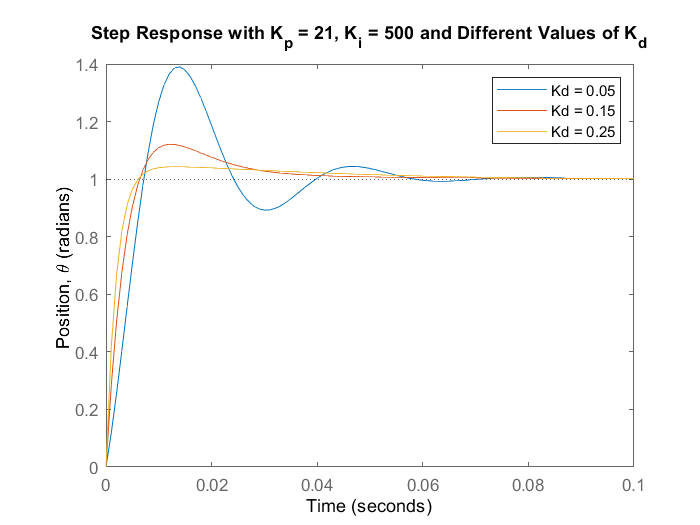
\includegraphics[width=7.5cm]{fig/PIDpos.png}
			\end{center}
		\end{column}
	\end{columns}
\end{frame}

\begin{frame}
	\frametitle{Embedded Video}  
	\begin{center}
		\movie{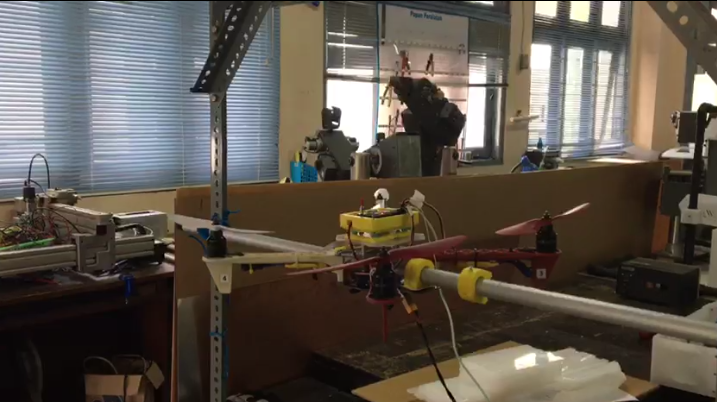
\includegraphics[scale=0.5]{video/videoThumbnail.png}}{video/Quadcopter tuning PID.mp4}
	\end{center}
\end{frame}

\begin{frame}
	\frametitle{Embedded Video}  
	\begin{center}
		\movie{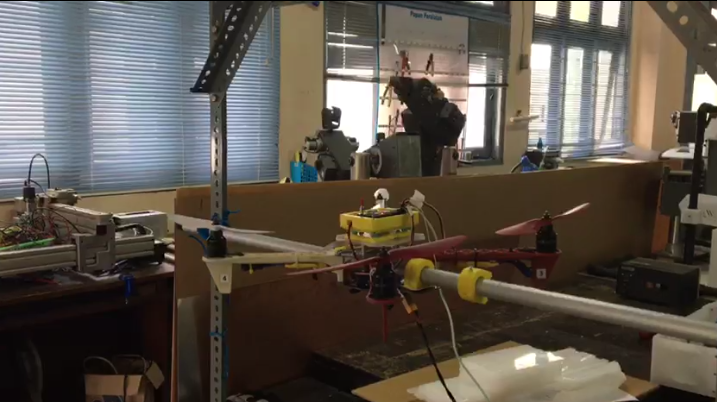
\includegraphics[width=13cm, height=7.5cm]{video/videoThumbnail.png}}{video/Quadcopter tuning PID.mp4}
	\end{center}
\end{frame}

\begin{frame} 
	\frametitle{References}        
	\nocite{*}
	\bibliography{bibfile}
\end{frame}



\begin{frame}
	\frametitle{Q\&A}
	\begin{figure}
		\centering
		
\includegraphics[scale=1]{fig/QandA.jpg}
	\end{figure}
\end{frame}

  
\end{document}